% theory-validation report (JBES revision add-on). Built by build_report.sh.
% Standalone; reuses the paper's \best/\second highlighting conventions.
\documentclass[11pt]{article}
\usepackage[margin=0.9in]{geometry}
\usepackage[table]{xcolor}
\usepackage{booktabs}
\usepackage{graphicx}
\usepackage{float}
\usepackage{amsmath,amssymb}
\usepackage{caption}
\usepackage{hyperref}

% Paper highlighting conventions.
\definecolor{bestgreen}{HTML}{00A651}
\definecolor{secondgreen}{HTML}{A8E6B0}
\newcommand{\best}[1]{\cellcolor{bestgreen}{\textbf{#1}}}
\newcommand{\second}[1]{\cellcolor{secondgreen}{#1}}

\newcommand{\fig}[3]{%
  \begin{figure}[htbp]\centering
  \IfFileExists{figs/#1}{\includegraphics[width=\linewidth]{figs/#1}}{\textit{[missing figs/#1]}}
  \caption{#2}\label{#3}\end{figure}}
\newcommand{\tab}[3]{%
  \begin{table}[htbp]\centering
  \IfFileExists{tables/#1}{\input{tables/#1}}{\textit{[missing tables/#1]}}
  \caption{#2}\label{#3}\end{table}}

\title{MPTE: Theory-Validation Simulation\\\large Results report (internal, for discussion)}
\author{}
\date{\today}

\begin{document}
\maketitle

\section{What this validates}
The inferential theory (Theorems 1--3) is derived for the \emph{linear} MPTE estimator: PCA on
the attention-weighted panel $\widetilde Z = B Z A_z$ with fixed operators $B$, $A_z$. This report
validates that estimator on a controlled union-factor linear DGP with known ground truth, and
bridges it to the nonlinear model. Four experiments: E1 consistency (Theorem~1), E2 coverage
(Theorems~2--3), E3 efficiency from transfer learning, E4 nonlinear bridge.

\paragraph{Model note: recovering the two attention operators.} The theory uses two operators, a
temporal $B$ ($T\times T$) that reweights time and a cross-sectional $A_z$ ($N\times N$) that
reweights variables. A single self-attention layer produces only \emph{one} square matrix, over
whatever we treat as its tokens: attend over the $T$ time rows and we get a $T\times T$ matrix
($B$); attend over the $N$ variable columns and we get an $N\times N$ matrix ($A_z$). One attention
therefore sees one axis only. The empirical pipeline flattens the whole panel into one long token
stream, runs one large attention over it, and recovers $B$ and $A_z$ afterward by averaging that
attention over variables and over time. At the sizes needed to trace asymptotic rates the
flattening is infeasible: a flattened $T\times N$ panel has $T\!\cdot\!N$ tokens and a
$(T\!\cdot\!N)^2$ attention, for example $160{,}000$ tokens and $2.56\times10^{10}$ entries at
$N=T=400$. We therefore use \emph{axial} attention: one attention over the $N$ columns yields $A_z$
and one attention over the $T$ rows yields $B$, directly and at cost $N^2+T^2\approx3.2\times10^5$.
This produces the same two operators the paper defines, obtained directly rather than by averaging a
flattened map. The value map is fixed to the identity ($W^v=I$, so $V=Z$): the attention reweights
the panel $Z$ itself, which keeps $\widetilde Z=BZA_z$ an approximate factor model in the same
factors and loadings, so PCA on $\widetilde Z$ recovers them.

\paragraph{Setup.} The data-generating process is the union-factor linear model of the design
note ($k=4$ factors, $N_x{:}N_y=2{:}1$, iid idiosyncratic noise). Every quantity averages over
$2000$ Monte Carlo replications: per $(T,N)$ cell in E1 (grid $N=T\in\{80,160,320,640,1000\}$), in
E2 and E3, and over $2000$ out-of-sample panels in E4 (at $N=T=300$).

\section{E1 --- Consistency (Theorem 1)}
Theorem~1 gives consistency of the factor, loading, and common-component estimates. We track the
common component $C=F\Lambda^\top$, the rotation-free combination of the factor and loading
estimates: it needs no rotation alignment and summarizes both in one quantity. We report its
relative error $\|\widehat C - C\|_F^2/\|C\|_F^2$ as the panel grows along $N=T$. The relative form
is scale-invariant, so it is comparable across operator arms, whereas the absolute error confounds
estimation quality with the operator-dependent scale of the target $C=BCA_z$. Consistency requires
the relative error to decline toward zero, and a log-log slope near $-1$ matches the classical PCA
rate $1/T+2/N$.

We report three operator arms, each grounded in the paper. The oracle arm fixes $A_z=I$ and $B=I$,
the pure-theory reference. The parameter-free arm uses the paper's simplest attention, $Q=K=Z$, so
that $A_z=\mathrm{softmax}(Z^\top Z/\cdot)$ carries no learned projection. The learned arm reads the
frozen, scaled attention off the trained linear model, estimated on a separate panel and then held
fixed, the sample-splitting convention of the paper's Remark~1. All three arms converge at a slope
near one (Figure~\ref{fig:e1}, Table~\ref{tab:e1slope}), so they agree, which is the property the
design asks for: the data-driven operators inherit Theorem~1 at the same rate as the oracle.

\paragraph{A note on Assumption A.7.} For the two data-driven arms the cross-sectional operator
norm $\|A_z\|_{\mathrm{op}}$ grows with $N$ rather than staying bounded, so A.7 as stated does not
hold along this path. The convergence rate is nevertheless unaffected, as panel (d) read against
panels (a)--(c) shows. We read this as evidence that A.7 is sufficient but stronger than necessary
in these designs. Whether it can be relaxed to a slowly growing operator norm, with the rate
re-derived, is a question for the theory that we leave open here.
\fig{e1_rate.pdf}{E1: relative estimation error against $N=T$ on log-log axes for (a) the common
component $C$, (b) the factors $F$, and (c) the loadings $\Lambda$, each with a slope near $-1$ for
all three operator arms; (d) the cross-sectional operator norm $\|A_z\|_{\mathrm{op}}$, which grows
for the data-driven arms while the rates in (a)--(c) hold.}{fig:e1}
\tab{e1_slope.tex}{E1: fitted slope of the relative error against $N$ (target $-1$) for the common
component, factors, and loadings, per operator arm, with the operator norm at the largest $N$.}{tab:e1slope}

\section{E2 --- Coverage / asymptotic normality (Theorems 2--3)}
Empirical coverage of CIs for the $Y$-strong common component $C_{y,i,t}$, using the analytic
plug-in variance from the paper. For the baseline iid DGP the long-run covariances collapse to
$\Omega=\sigma^2\Sigma_{F,y}$, $\Xi=\sigma^2\Sigma_{\Lambda,y_s}$, and we studentize with the general
Theorem-3(iii) variance $\mathrm{Var}(\widehat C-C)=\sigma^2_{F}/N+\sigma^2_{\Lambda}/T$ (the F- and
$\Lambda$-dominant cases are its limits). Coverage is near nominal in all three regimes
(Table~\ref{tab:e2cov}) and the studentized statistic is standard normal (Figure~\ref{fig:e2qq}).
\tab{e2_coverage.tex}{E2: empirical coverage of $90\%$/$95\%$ CIs and the studentized-statistic sd, by regime.}{tab:e2cov}
\fig{e2_qq.pdf}{E2: QQ plot of the studentized $C_{y,i,t}$ against $\mathcal N(0,1)$ (mixed regime).}{fig:e2qq}

\section{E3 --- Efficiency from transfer learning}
The joint $(X,Y)$ estimator of $C_{y,i,t}$ is more precise than the $Y$-only estimator; the gain
grows with the auxiliary size $N_x$ and saturates because only one factor is shared
(Figure~\ref{fig:e3}, Table~\ref{tab:e3}).
\fig{e3_efficiency.pdf}{E3: MSE ratio (Y-only / joint) vs.\ $N_x$.}{fig:e3}
\tab{e3_ratio.tex}{E3: joint vs.\ Y-only common-component MSE and their ratio.}{tab:e3}

\section{E4 --- Nonlinear bridge}
On linear-truth data we ask whether the nonlinear model builds the factor representation the theory
describes (Figure~\ref{fig:e4}). We measure two subspaces against the true attended factors
$F^{(B)}=BF$ by canonical correlation: the nonlinear model's $k$-dim latent, and the linear PCA
estimator's factors. The linear estimator recovers the full attended factor space. The nonlinear
model, trained on a
single-target forecast objective with a deliberately minimal architecture, recovers the
target-relevant direction strongly (leading canonical correlation $\approx 0.98$) while leaving the
orthogonal factors to the linear estimator, since a single-target objective only needs the direction
that predicts its target. The forecast-accuracy equivalence between the nonlinear model and the
linear ablation is the paper's Table~1 result; here we add the factor-space statement against known
ground truth for the target signal.
\fig{e4_cca.pdf}{E4: canonical correlations with $F^{(B)}$, nonlinear latent vs.\ linear PCA. The
nonlinear model recovers the leading, target-relevant factor; the linear estimator recovers the full
space.}{fig:e4}

\section{Learned operators}
Figure~\ref{fig:ops} shows the frozen cross-sectional operator $A_z$ and temporal operator $B$ read
off the trained linear model on one panel. The attention concentrates on a few variables and time
points, the bright stripes, which is the structure behind the operator norm that grows with $N$ in
Figure~\ref{fig:e1}(d).
\begin{figure}[ht]\centering
\IfFileExists{figs/operators.pdf}{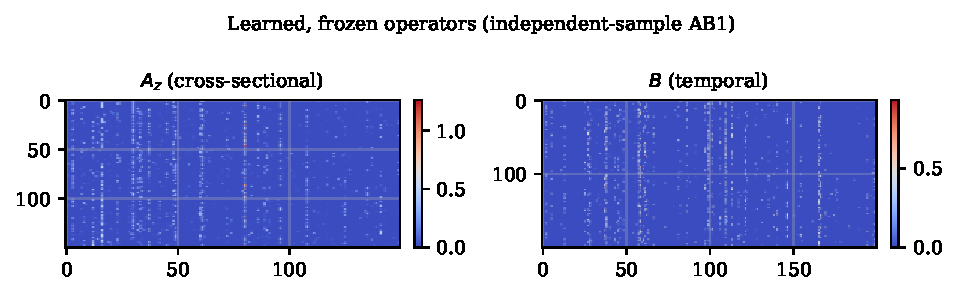
\includegraphics[width=\linewidth]{figs/operators.pdf}}{\textit{[missing figs/operators.pdf]}}
\caption{Learned, frozen $A_z$ ($N\times N$) and $B$ ($T\times T$) from the independent-sample
linear model.}\label{fig:ops}\end{figure}

\clearpage
\section*{Addition after July 2nd}
The three exhibits below were added after the first read, following the July email. Each answers
one request directly, and each is reported as it comes out, including the two where the clean
picture does not appear. We think the honest version is the informative one.

\subsection*{A1. E1: error against the theoretical rate $\bar\alpha$}
The request was to plot the factor and loading errors against the theoretical rate $\bar\alpha$
rather than against $N$. Figure~\ref{fig:e1alpha} shows the relative errors on log-log axes against
$\bar\alpha=1/T+2/N$. For the oracle the two move together on the slope-1 line, exactly as
Theorem~1 asks. For the two data-driven arms the points scatter off the line: their realized
$\bar\alpha$ absorbs the cross-sectional operator norm $\|A_z\|_{\mathrm{op}}$, which grows with
$N$ and is non-monotone across the grid, so $\bar\alpha$ is no longer the clean scalar the plot
needs on its horizontal axis. This is the same fact the main-text A.7 note reports, seen from the
rate side. The consistency claim itself is untouched: the error-against-$N$ panels
(Figure~\ref{fig:e1}) stay on slope $-1$ for every arm, so the data-driven operators do converge at
the full rate. We keep both views and read them together.
\fig{e1_error_vs_alpha.pdf}{Addition: relative error against the theoretical rate $\bar\alpha$ on
log-log axes for (a) the factors and (b) the loadings, one series per operator arm, with a slope-1
reference. The oracle follows the reference; the data-driven arms scatter because their realized
$\bar\alpha$ carries the growing operator norm.}{fig:e1alpha}

\subsection*{A2. E4: block-wise factor recovery}
The request was to split the E4 canonical correlations by factor block: the $Y$-strong block
$F^{(B)}_S$, which the target loads on, against the rest block $F^{(B)}_R$ of $X$-only factors.
Table~\ref{tab:e4block} reports both blocks for the nonlinear latent and for the linear PCA
factors. The linear estimator recovers both blocks near one, as a full-panel estimator should. The
nonlinear latent recovers the leading $Y$-strong direction strongly (cc$_1\approx0.98$) but not the
second $Y$-strong direction, and it also correlates with the rest block. The reason is that the
latent is a linear read-out of the whole attended panel $\widetilde Z$, and $\widetilde Z$ carries
the $X$ columns, so the rest factors sit inside the representation regardless of its dimension. We
also tried shrinking the latent to $k=2$; that made the $Y$-strong recovery worse, not sharper, and
did not separate the blocks. So the defensible reading of E4 is a statement about the
target-relevant \emph{direction} the forecast objective identifies, not about isolating a full
$Y$-strong \emph{block}. A clean block statement would need a different probe, the subspace the
forecast head actually uses, or a design where the target loads on the whole block.
\tab{e4_block.tex}{Addition: block-wise canonical correlations with the true attended factors, the
$Y$-strong block $F^{(B)}_S$ against the rest block $F^{(B)}_R$, for the nonlinear latent and the
linear PCA factors ($k=4$, $N=T=300$).}{tab:e4block}

\subsection*{A3. E2: coverage under the learned operators}
The main-text E2 uses the oracle operators, where the assumptions hold exactly. The request was to
add the learned, frozen operators alongside. Table~\ref{tab:e2both} reports both. The oracle stays
near nominal in all three regimes; the learned arm under-covers sharply, with the studentized
statistic spreading well past unit variance. The cause is specific: the analytic plug-in uses the
iid collapse $\Omega=\sigma^2\Sigma_{F,y}$, $\Xi=\sigma^2\Sigma_{\Lambda,y_s}$, but once the panel
is passed through a concentrated $A_z$ the attended noise $B\,e\,A_z$ is no longer iid, so that
collapse is misspecified and the interval is the wrong width. This is not a bug to tune away: it is
the finite-sample counterpart of the general Theorem-3 variance with the full $\Omega$, $\Xi$, and
it is the piece that pairs with the A.7 relaxation. Reporting both arms makes the boundary explicit,
the theory is calibrated where its assumptions hold and needs the general variance where the
operators concentrate.
\tab{e2_both_arms.tex}{Addition: empirical coverage of the $90\%$/$95\%$ CIs and the
studentized-statistic sd, oracle operators against learned frozen operators, by regime. The oracle
$95\%$ cells are highlighted; the learned arm's operator norm is $\|A_z\|_{\mathrm{op}}\approx4.5$
(F-dominant), $10.1$ ($\Lambda$-dominant), $8.8$ (mixed).}{tab:e2both}

\clearpage
\section*{Addition after July 6th}
This round follows the four items of the July email, in order. The first two are settled and we
adopt the reading proposed there. The third is the coverage work, where we ran all three checks. The
fourth is the projected operator arm, which we correct into a blend and, once it points the way, close
the coverage story with a boundary exhibit in the paper's own quantities.

\subsection*{B1. E1 axis: the realized rate $\bar\alpha$ per arm}
The horizontal axis of Figure~\ref{fig:e1alpha} is each arm's own realized three-term rate
$\bar\alpha$, computed from that arm's operators; it equals $1/T+2/N$ only at the oracle, where
$A_z=I$ and $B=I$. Read this way, Theorem~1 is an upper bound, error $=O_P(\bar\alpha)$, so points
on or below the slope-1 line are what it permits. The bound is sharp at the oracle, where A.7 holds,
and conservative under the concentrated data-driven operators, where the slack sits in the middle
term of $\bar\alpha$.

\subsection*{B2. E4 blocks: a one-dimensional identified set}
With a single-target forecast objective the identified set is one-dimensional: the forecast needs
only the $\Lambda_i$ combination of the strong factors, so a leading canonical correlation near
$0.98$ on one $Y$-strong direction, and no more, is what the theory predicts. The pickup on the rest
block is something the theory neither requires nor forbids. This is the statement we attach to
Table~\ref{tab:e4block}.

\subsection*{B3. Coverage under the learned operators}
We ran the three checks. Table~\ref{tab:e2gate} collects coverage for the oracle and four learned
variants (raw, block-restricted, clipped, blend) under three variance channels: the iid plug-in, the
feasible general plug-in, and the Monte Carlo sd, alongside the A.7 quantities $\|A_z\|_{\mathrm{op}}$
and $\mathrm{PR}/N$ (the participation ratio $\mathrm{PR}=\mathrm{tr}(A_z^\top A_z)^2/
\|A_z^\top A_z\|_F^2$, the effective dimension; $\mathrm{tr}/N=1$ for all by the scaling).

\emph{(a) Re-studentize with the Monte Carlo variance.} Dividing the same learned-arm draws by the
sd measured in simulation restores the distributional shape, the studentized statistic is close to
normal with the QQ bulk on the line (Figure~\ref{fig:e2qq6}) and coverage near nominal in the F- and
$\Lambda$-dominant regimes, but a location term remains: coverage still falls short, unevenly across
regimes (Table~\ref{tab:e2gate}, MC column). So the width was part of the problem; a residual bias in
the common component is the rest.

\emph{(b) Block restriction.} The E2 operators were not block-restricted, so we reran with the
X-to-Y cross terms zeroed. The collapse under the iid plug-in barely moves (Table~\ref{tab:e2gate},
learned rows), so it is not identification leakage from the $X$ block; it is the interval itself.

\emph{(c) The feasible general plug-in.} The attended noise $\widetilde e=B e A_z$ has a known
covariance up to one scalar, $\mathrm{Cov}(\widetilde e_{ti},\widetilde e_{sj})=
\sigma^2 (BB^\top)_{ts}(A_z^\top A_z)_{ij}$, so we estimate $\sigma^2$ from the PCA residuals and
rebuild the two score covariances with $(A_z^\top A_z)$ and $(BB^\top)$ inserted where the iid
collapse used identities. This is the Theorem-3 variance specialized to our frozen-operator design.
It reduces to the iid plug-in at the oracle exactly, and it recovers most of the width the iid
collapse discards, but on the raw and block-restricted arms it stops short of nominal.

The reason it stops short is a finite-sample bias that does not close as the panel grows, and it is
a statement in the paper's own quantities. Figure~\ref{fig:e2bias} sweeps $N=T$ for the learned arm
and reports, averaged over operator seeds and cells, the standardized bias and the coverage under the
Monte Carlo and general widths, next to $\sqrt N\,\bar\alpha$. The middle term of $\bar\alpha$ equals
$1/\mathrm{PR}$, so a bounded participation ratio makes $\bar\alpha$ stall and $\sqrt N\,\bar\alpha$
grow rather than vanish; the Theorem 2--3 growth conditions $\sqrt T\,\bar\alpha\!\to\!0$ and
$\sqrt{N_{\mathrm{eff}}}\,\bar\alpha\!\to\!0$ therefore fail, and the $o_p(1)$ remainders surface as
exactly the non-vanishing bias we measure. The single-target attention concentrates on a bounded set
of hub variables, so $\mathrm{PR}/N$ keeps shrinking and the effective dimension does not grow with
$N$. This does not contradict E1: the Frobenius-norm error in Figure~\ref{fig:e1} is carried by the
high-signal hub cells the attention favors, while the $Y$-block target cells keep a small relative
bias.
\tab{e2_gate.tex}{Addition: E2 coverage of the $95\%$ CI by regime and operator arm, with the A.7
quantities $\|A_z\|_{\mathrm{op}}$ and $\mathrm{PR}/N$, under the iid plug-in, the feasible general
plug-in, and the Monte Carlo sd. The clip and blend arms apply the same projection to the temporal
operator $B$; the general-plug-in cells for the arms inside the theory's domain (oracle and blend)
are highlighted.}{tab:e2gate}
\fig{e2_learned_qq.pdf}{Addition: QQ of the learned-arm studentized statistic (mixed regime) under
the iid plug-in, the general plug-in, and the Monte Carlo sd. The iid tails fan out; the general and
Monte Carlo channels pull the bulk onto the line but leave a residual off-center from the
finite-sample bias.}{fig:e2qq6}
\fig{e2_bias_sweep.pdf}{Addition: (a) coverage against $N=T$ under the Monte Carlo and general
widths, both plateauing below the nominal $0.95$; (b) the standardized bias and the growth product
$\sqrt N\,\bar\alpha$, neither of which vanishes, because the learned operator stays concentrated
(its participation ratio does not grow with $N$).}{fig:e2bias}

\subsection*{B4. The projected arms: clip and blend}
A.7's two halves are jointly an anti-concentration condition. If $\|A_z\|_{\mathrm{op}}\le\kappa$ and
$\mathrm{tr}(A_z^\top A_z)/N=c_A$, then $\mathrm{PR}/N\ge c_A/\kappa^2$; each half alone is satisfiable
by a concentrated operator, and the two failing arms show it. The raw arm keeps the trace half by
scaling but its op-norm grows, so it fails the norm half. We then try two projections that are
deterministic functions of the frozen operator, so the sample-splitting convention is intact, and we
apply each to \emph{both} operators, since the temporal $B$ is concentrated on the same footing as
$A_z$ and drives the loading-CLT term.

The \emph{clip} caps the singular values at $\kappa=3$ and re-applies the trace scaling. For an
effectively low-rank spectrum this has no fixed point: clipping removes top mass but cannot create
the tail mass the trace half needs, so the rescale nudges the op-norm back above $\kappa$ and the arm
lands on the A.7 boundary, $\mathrm{PR}/N$ just above $c_A/\kappa^2$ (Table~\ref{tab:e2gate}).
Coverage improves but stops short. The \emph{blend} adds the missing tail mass: clip at $\kappa_0=3$,
add $\delta I$ with $\delta=1$, then trace-rescale once. It is a shrinkage of the learned attention
toward the identity, giving every variable a baseline self-weight, and it lands comfortably inside the
domain, $\mathrm{PR}/N\approx0.35$ with the op-norm at or below $3$. Under the general plug-in the
blend arm is near nominal in all three regimes (Table~\ref{tab:e2gate}, blend rows), and its Monte
Carlo coverage is nominal, so it validates the domain where the clip only reaches its edge.

Fixing both axes is necessary, and which axis binds is regime-dependent in exactly the way the two
CLT terms predict. Blending $A_z$ alone nearly closes the F-dominant regime, where small $N$ makes
the factor-CLT term (carrying $A_z$) dominant, but not the $\Lambda$-dominant regime; blending $B$
alone does the reverse, closing $\Lambda$-dominant, where small $T$ makes the loading-CLT term
(carrying $B$) dominant; only blending both closes the mixed regime. The binding quantity is the pair
of anti-concentration conditions, one per axis.

\subsection*{B5. The boundary in theorem-native units}
Figure~\ref{fig:e2delta} sweeps the blend shrinkage $\delta$ from $0$, the concentrated end where the
blend reduces to the clip, toward $5$, where it converges to the identity, applied to both operators,
and plots the general-plug-in coverage against the realized effective rank $\mathrm{PR}/N$
(equivalently the middle term of $\bar\alpha$, since it equals $1/\mathrm{PR}$). As $\delta$ lifts
$\mathrm{PR}/N$ through the A.7 threshold $c_A/\kappa_0^2$, coverage climbs to nominal: inference
switches on precisely as the operators re-enter the theory's domain. The boundary is a single curve in
the paper's own quantity.
\fig{e2_delta_sweep.pdf}{Addition: general-plug-in coverage of the blend arm against the effective
rank $\mathrm{PR}/N$ as the shrinkage $\delta$ grows from $0$ to $5$ (both operators blended), one
curve per regime, with the A.7 threshold $c_A/\kappa_0^2$ marked. Coverage reaches nominal as the
effective rank is restored.}{fig:e2delta}

\end{document}
